\chapter{BẢN VẼ SCHEMATIC}
\section{Các cụm chức năng trên bản vẽ schematic}

\subsection{Cụm nguồn động cơ}
\begin{figure}[H]
    \centering
    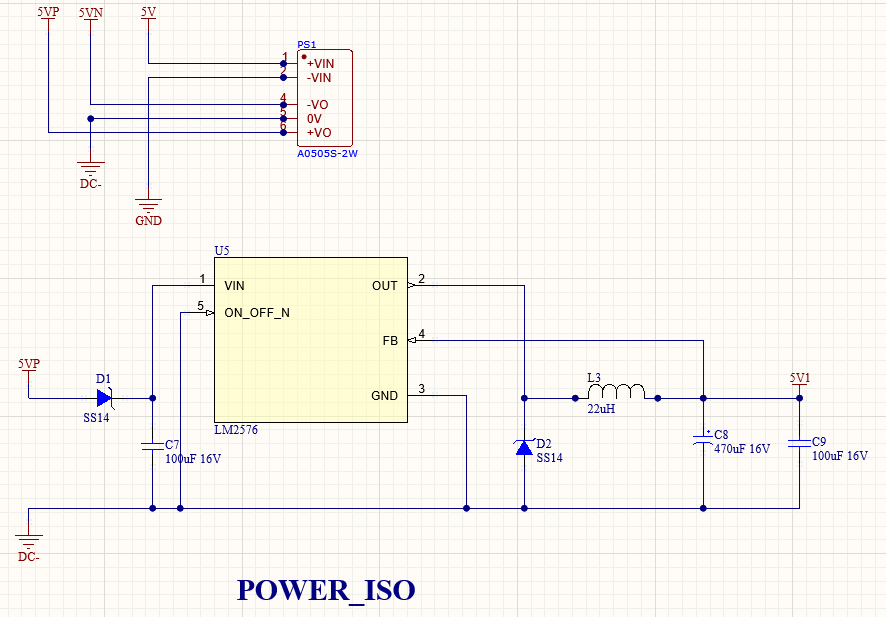
\includegraphics[width=1\textwidth]{pictures/power_iso.png}
\end{figure}
\begin{itemize}
    \item Ở cụm nguồn trên, sử dụng module nguồn cách ly DC-DC A0505S-2W để chuyển đổi nguồn và có 
    tác dụng cách ly điện áp. Cụ thể module nhận điện áp 5V ở đầu vào (chân +VIN) sau đó chuyển đổi 
    thành 2 nguồn 5VP và 5VN ở đầu ra (nguồn 5VP tương ứng với chân +VO và 0V, nguồn 5VN tương ứng với 2 chân -VO và 0V). Tuy nhiên dòng tải tối đa module này có thể cung cấp chỉ khoảng từ 400mA đến 500mA.
    \item Ngoài ra LM2576 là một IC điều chỉnh điện áp hạ áp, trong cụm chức năng này, IC LM2576 thực hiện lấy điện áp 5V từ đầu ra
    của module A0505S-2W làm điện áp đầu vào để ổn định điện áp ở mức 5V đồng thời cung cấp dòng lớn (3A), phù hợp cho yêu cầu của các tải phía sau.
\end{itemize}

\subsection{Cụm điều khiển động cơ}
\begin{figure}
    \centering
    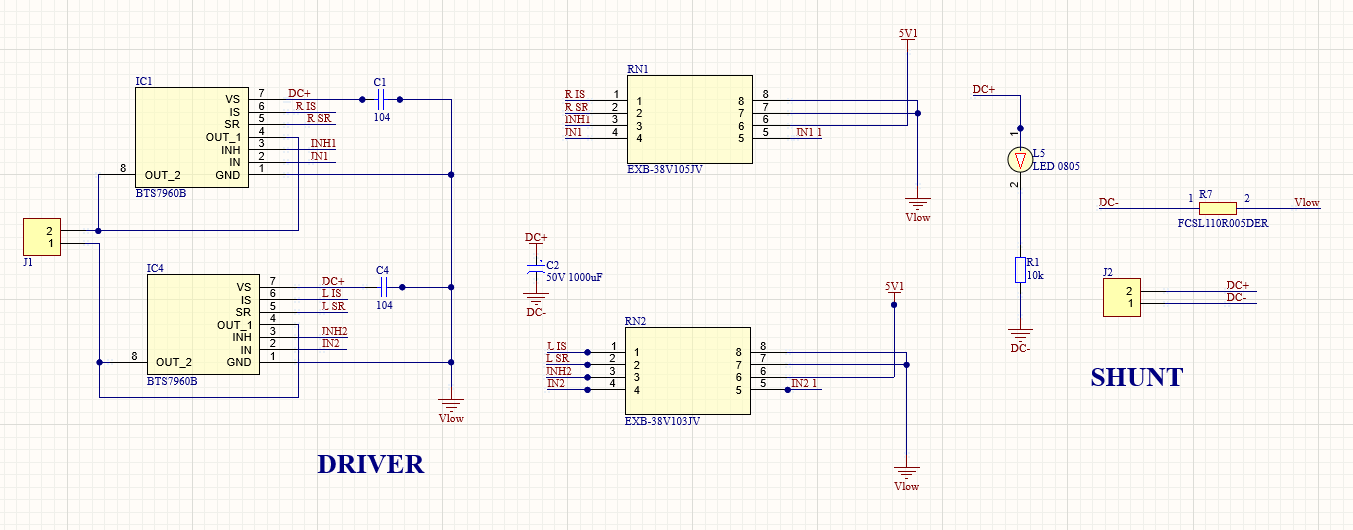
\includegraphics[width=1\textwidth]{pictures/driver.png}
\end{figure}
\begin{itemize}
    \item Trong cụm DRIVER sử dụng 2 IC BTS7960B để tạo thành một mạch cầu H điều khiển hướng quay và tốc độ động cơ bằng cách thay đổi trạng thái 2 chân INH và IN.
    \item RN1, RN2 (EXB-38V105JV): các mạng điện trở (resistor network) dùng để điều chỉnh tín hiệu điều khiển từ bộ vi điều khiển (MCU) xuống các chân INH và IN của BTS7960B.
    \item Tụ gốm C1 và C4 100nF để lọc nhiễu ở chân cấp nguồn DC+.
    \item Tụ lọc lớn C2 1000uF để ổn định nguồn DC+.
    \item Header J1 dùng để giao tiếp, nhận tín hiệu điều khiển từ MCU (INH1, INH2, IN1, IN2).
\end{itemize}


\section{Bản vẽ schematic hoàn chỉnh}
\begin{figure}[H]
    \centering
    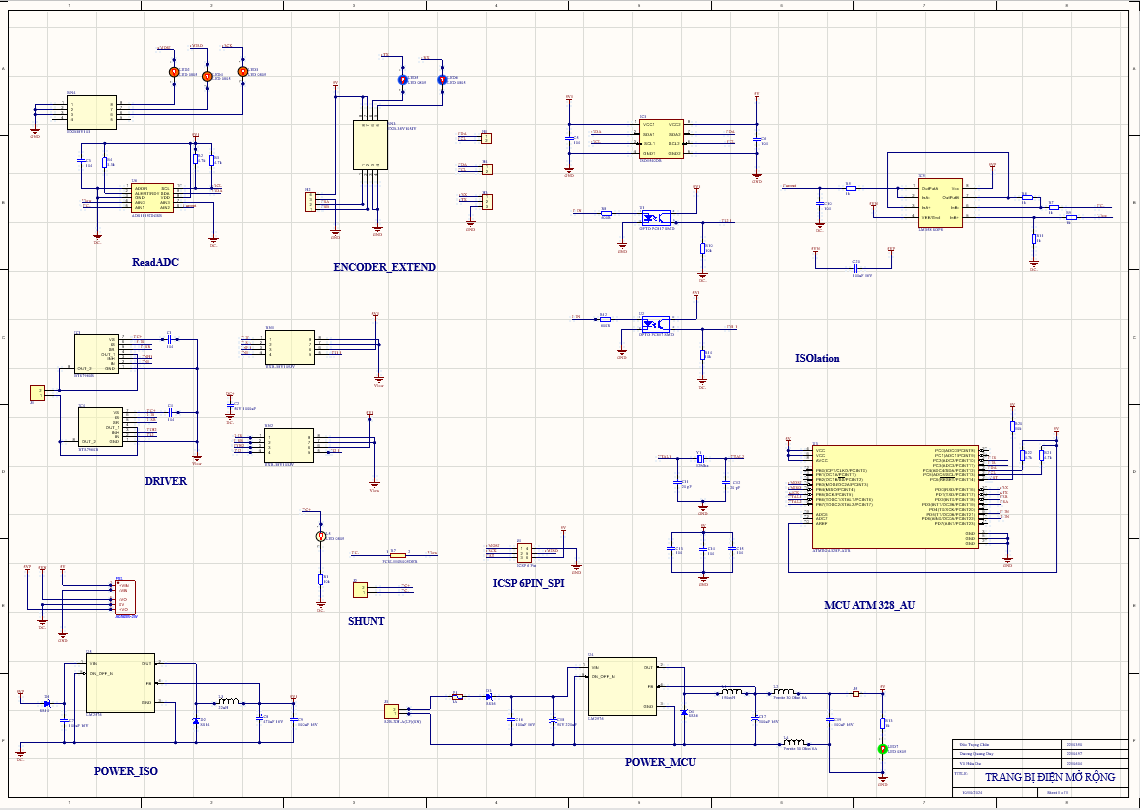
\includegraphics[width=1\textwidth]{pictures/ISO_current.png}
    \caption{Bản vẽ schematic hoàn chỉnh}
\end{figure}
\cleardoublepage
